\chapter{METODOLOGI PENELITIAN}
%\section{Tempat dan Jadwal Kegiatan Penelitian}
%Dalam melaksanakan sebuah penelitian, perencanaan waktu merupakan komponen kritis yang memastikan alur penelitian dapat berjalan dengan terstruktur dan sistematis. Gambar \ref{fig:jadwal-penelitian} menyajikan jadwal penelitian yang telah dirancang untuk penelitian ini. Jadwal tersebut mencakup rentang waktu mulai dari September 2023 hingga April 2024 dan menguraikan berbagai kegiatan yang akan dilakukan selama periode tersebut. Selanjutnya, penelitian ini akan dilaksanakan di Laboratorium Komputer, Institut Teknologi Sumatera.
%
%\begin{figure}[h!]
%    \centering
%    \includegraphics[width=1\textwidth]{figures/ch03/Timeline-2.png}
%    \caption{Jadwal Penelitian}
%    \label{fig:jadwal-penelitian}
%\end{figure}


\section{Alur Penelitian}
Adapun diagram alir penelitian ini ditunjukkan pada Gambar \ref{fig:diagram alir} terdapat enam tahapan. Langkah awal yang dilakukan pada penelitian ini adalah melakukan identifikasi masalah, yaitu proses mencari, menghimpun, serta menemukan permasalahan yang nantinya akan diselesaikan. Setelah melakukan identifikasi masalah, langkah selanjutnya adalah studi literatur. Studi literatur adalah tahapan untuk mencari solusi dari permasalahan yang sebelumnya sudah kita definisikan. Pencarian solusi ini dapat melalui membaca referensi ilmiah terdahulu, baik melalui jurnal, buku, dokumentasi resmi, tesis, dan lain-lain. Tahapan ini akan memberikan pemahaman mendasar mengenai permasalahan yang sudah didapatkan sebelumnya. 
        
\begin{figure}[h!]
    \centering
    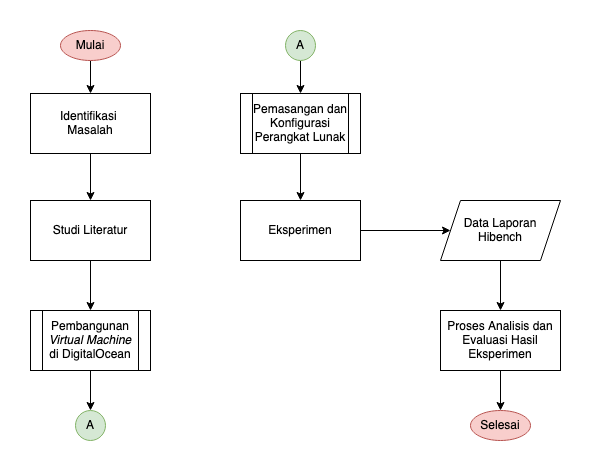
\includegraphics[width=0.9\textwidth]{figures/ch03/Diagram Tugas Akhir.png}
    \caption{Diagram Alir Penelitian}
    \label{fig:diagram alir}
\end{figure}

\newpage
Kemudian, penelitian ini akan dilanjutkan pada tahap membangun \textit{virtual machine} di DigitalOcean. DigitalOcean adalah perusahaan penyedia layanan awan \textit{Infrastructure as a Service} (IaaS) yang memberikan banyak pilihan kepada pengguna untuk menggunakan berbagai jenis layanan sesuai dengan kebutuhan, salah satunya yaitu \textit{virtual machine}. \textit{Virtual Machine} tersebut dapat dihentikan atau dihapus kapanpun saat tidak lagi diperlukan. Ketika infrastruktur sudah siap digunakan, penelitian dilanjutkan ke tahap pemasangan perangkat lunak, seperti Hadoop, Spark, dan HiBench. Selanjutnya dilakukan eksperimen pada beban kerja \textit{Micro Benchmarks}. Akhirnya, hasil dari eksperimen akan digunakan untuk proses analisis dan evaluasi.

\section{Identifikasi Masalah dan Studi Literatur}
Langkah awal penelitian ini adalah identifikasi masalah dan studi literatur. Identifikasi masalah dapat dipahami sebagai tahapan mendefinisikan masalah sehingga masalah tersebut dapat terukur dan jelas untuk dijadikan landasan dalam latar belakang penelitian. Setelah masalah berhasil diidentifikasi, langkah selanjutnya adalah studi literatur yang mana dalam proses ini dilakukan pengumpulan berbagai macam informasi, referensi, dan konsep dasar yang menjadi landasan dasar dari penelitian. Langkah ini dapat dilakukan melalui membaca artikel ilmiah pendukung, buku-buku yang ditulis oleh para ahli, dan jika berkaitan dengan pemrograman dapat melihat dari dokumentasi resmi. Pada tahap ini juga dilakukan analisis terhadap penelitian terdahulu dan dibandingkan dengan identifikasi masalah yang didapatkan untuk membuka celah penelitian baru sehingga penelitian ini dapat bermanfaat. 

\section{Membangun \textit{Virtual Machine} di DigitalOcean}
Konfigurasi perangkat keras merupakan aspek penting dalam mengevaluasi kinerja aplikasi \textit{big data} berbasis Hadoop dan Spark. DigitalOcean, sebagai penyedia layanan infrastruktur sebagai layanan (IaaS), memberikan pengguna kebebasan penuh untuk membuat, mengonfigurasi, dan mengelola berbagai infrastruktur yang telah disediakan. Dalam konteks penelitian ini, diperlukan penggunaan mesin virtual, yang dalam DigitalOcean dikenal sebagai "\textit{Droplets}," yang memungkinkan untuk menyesuaikan berbagai aspek seperti sistem operasi, kapasitas penyimpanan, jumlah prosesor, dan parameter lainnya sesuai dengan kebutuhan spesifik penelitian.

\begin{table}[h!]
	\centering
	\caption{Konfigurasi Perangkat Keras}
	\begin{tabular}{l p{9cm}} 
		\toprule
		\textbf{Nama Parameter}    & \textbf{Nilai Parameter} \\ 
        \midrule
		\textbf{Lokasi Pusat Data} & Singapore - Datacenter 1 - SGP1               \\ 
		\textbf{Sistem Operasi}    & Ubuntu 20.04 (LTS) x64                        \\
		\textbf{Jenis \textit{Droplet}}     & Basic                                         \\ 
		\textbf{Prosesor}          & Premium AMD - 4 Core                          \\ 
		\textbf{Memori}            & 8 GB                                          \\ 
		\textbf{Penyimpanan}       & 160 GB NVMe SSD                               \\ 
        \bottomrule
	\end{tabular}
	\label{table:conf-hardware}
\end{table}
Penelitian ini mengadopsi mode \textit{pseudo-distributed} yang memungkinkan penggunaan hanya satu \textit{virtual machine} dalam konfigurasi \textit{single node}. Walaupun hanya menggunakan satu \textit{virtual machine}, mode \textit{pseudo-distributed} memungkinkan setiap proses dalam klaster beroperasi secara independen, menciptakan lingkungan di mana semua proses berjalan mandiri satu sama lain. Hal ini memungkinkan untuk lebih berfokus pada pengumpulan data dan analisis, tanpa perlu melakukan konfigurasi yang rumit terkait dengan pengaturan klaster. Spesifikasi perangkat keras yang digunakan untuk \textit{virtual machine} dalam mode \textit{pseudo-distributed} sesuai pada Tabel \ref{table:conf-hardware}. Penjelasan lengkap tentang pembuatan \textit{virtual machine} (VM) pada \textit{platform} DigitalOcean dan cara mengakses VM tersebut disajikan pada Lampiran \ref{appendix:A}.

\section{Pemasangan dan Konfigurasi Perangkat Lunak}
Pemasangan dan konfigurasi perangkat lunak merupakan hal yang krusial dalam penelitian ini. Perangkat lunak yang diperlukan ditunjukkan pada Tabel \ref{table:software-needs}.

\begin{table}[h]
	\centering
	\caption{Perangkat Lunak yang Dibutuhkan}
		\begin{tabular}{l p{9cm}} 
		\toprule
			\textbf{Perangkat Lunak} & \multicolumn{1}{c}{\textbf{Deskripsi}}                                                                                \\ 
            \midrule
			Ubuntu 20.04 LTS x64     & Sistem operasi Linux berbasis Ubuntu  \\ 
			Git                      & Sistem kontrol versi untuk mengelola perubahan dalam kode sumber perangkat lunak                                       \\
			Maven                    & Perangkat lunak manajemen proyek Java                            \\ 
			Java 8                   & \multirow{3}{*}{Bahasa pemrograman dasar}                                 \\ 
			Python 3.7               &                                                                                                                        \\
			Scala 2.11.8               &                                                                                                                        \\
			Hadoop 2.4                & Perangkat lunak pengolahan data terdistribusi untuk penyimpanan dan manajemen data besar                               \\ 
			Spark 2.1.3               & Kerangka kerja pemrosesan data terdistribusi yang berjalan di atas Hadoop                                              \\ 
			Hibench   & Alat yang digunakan untuk mengukur kinerja Hadoop dan Spark                                                            \\
			Dool   & Alat untuk melihat penggunaan \textit{resource} sistem                                                             \\
            \bottomrule 
		\end{tabular}
	\label{table:software-needs}
\end{table}


Alur kerja instalasi perangkat lunak dalam penelitian ini dapat dilihat pada Gambar \ref{fig:alurkerja-soft}. Pada gambar, terdapat tiga bagian utama, yaitu \textit{prerequisites} (perangkat lunak prasyarat) ditandai dengan warna biru, alat penyimpanan dan pemrosesan \textit{Big Data} ditandai dengan warna oren, dan alat untuk mengukur kinerja \textit{big data} ditandai dengan warna hijau. 

\begin{landscape}
\begin{figure}[h]
    \centering
    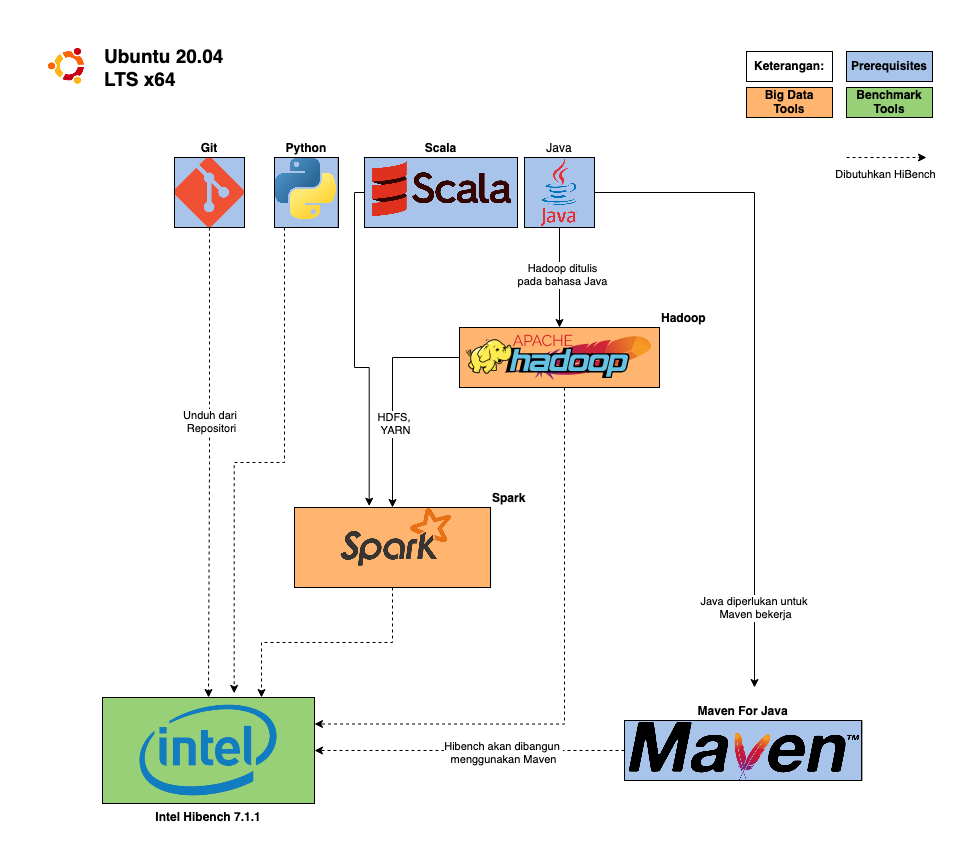
\includegraphics[height=0.65\linewidth]{figures/ch03/alurkerja-soft.png}
    \caption{Alur Instalasi Perangkat Lunak}
    \label{fig:alurkerja-soft}
\end{figure}
\end{landscape}

\subsection{Instalasi Perangkat Lunak Prasyarat}
Ada beberapa perangkat lunak yang perlu diimplementasikan sebelum memasang Hadoop, Spark, dan HiBench, yaitu:
\begin{enumerate}
	\item Ubuntu 20.04 LTS x64
	\item Git
	\item Java 8 dan Maven
	\item Python 3.7
	\item Scala 2.11.8
\end{enumerate}

Pemasangan dan konfigurasi perangkat lunak pada tahapan ini tidak membutuhkan urutan. Akan tetapi, pada penelitian ini dibuatkan alur untuk pemasangan dan konfigurasi perangkat lunak prasyarat seperti pada Gambar \ref{fig:prasyarat-flow}. Penjelasan lengkap mengenai tata cara instalasi dan konfigurasi perangkat lunak prasyarat ini disajikan pada Lampiran \ref{appendix:B}. 

\begin{figure}[h!]
    \centering
    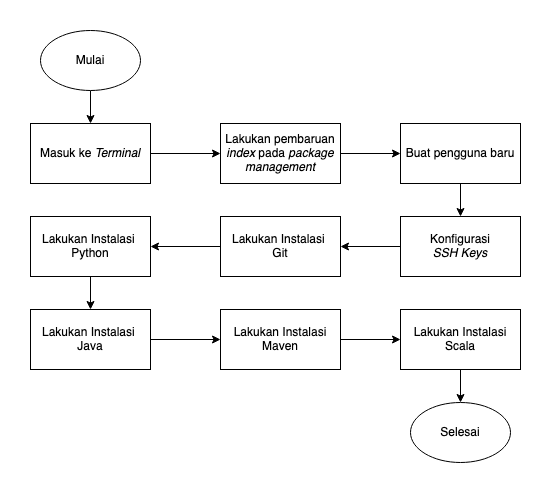
\includegraphics[width=0.9\textwidth]{figures/ch03/prasayarat-flow.png}
    \caption{Alur Instalasi Perangkat Lunak Prasyarat}
    \label{fig:prasyarat-flow}
\end{figure}

\subsection{Instalasi dan Konfigurasi Hadoop}
Hadoop adalah perangkat lunak \textit{open source} yang efektif dalam menyimpan dan memproses data dalam skala besar. Daripada menggunakan satu komputer besar untuk menyimpan dan memproses data, Hadoop memungkinkan pengklasteran beberapa komputer untuk menganalisis set data besar secara paralel dengan lebih cepat. Ada beberapa perangkat lunak prasyarat yang perlu dipasang sebelum menggunakan Hadoop. Setelah perangkat lunak prasyarat berhasil dipasang, Hadoop juga dapat dipasang mengikuti panduan lengkap pada Lampiran \ref{appendix:C}. 
Secara umum, alur yang harus dilakukan meliputi pengunduhan berkas Hadoop. Selanjutnya akan dilakukan pengubahan kepemilikan berkas ke \textit{user hdfsuser}. Karena Hadoop tidak mendukung IPv6, maka fitur ini perlu dimatikan juga. Alur pemasangan dan konfigurasi Hadoop lebih jelas sesuai dengan Gambar \ref{fig:hadoop-flow}.

\begin{figure}[h!]
    \centering
    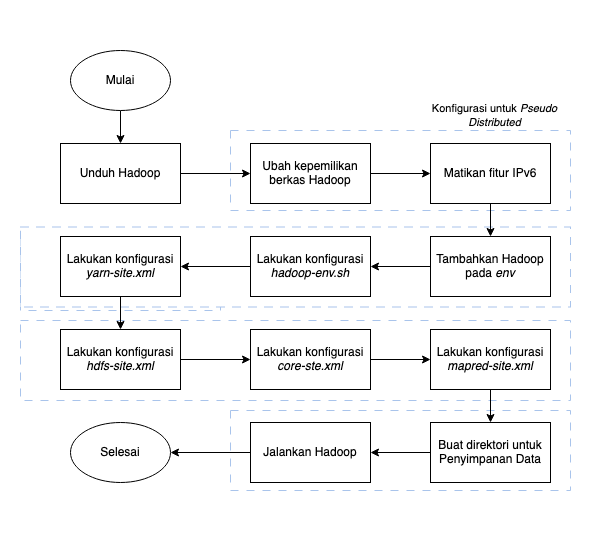
\includegraphics[width=0.9\textwidth]{figures/ch03/hadoop-flow.png}
    \caption{Alur Instalasi dan Konfigurasi Hadoop}
    \label{fig:hadoop-flow}
\end{figure}

\subsection{Instalasi dan Konfigurasi Spark}
Apache Spark adalah sebuah kerangka kerja pengolahan data terdistribusi yang sangat cepat dan efisien. Spark dan Hadoop memiliki hubungan yang erat. Spark dapat berjalan di atas \textit{Hadoop Distributed File System} (HDFS) dan dapat menggunakan Hadoop YARN sebagai manajer sumber daya. Oleh karena itu, instalasi Spark membutuhkan Hadoop sudah terpasang lebih dahulu. Alur pemasangan dan konfigurasi spark terlihat seperti pada Gambar \ref{fig:spark-flow}. Apabila Hadoop sudah berhasil terpasang, langkah selanjutnya adalah memasang Spark seperti pada Lampiran \ref{appendix:D}.

\begin{figure}[h]
    \centering
    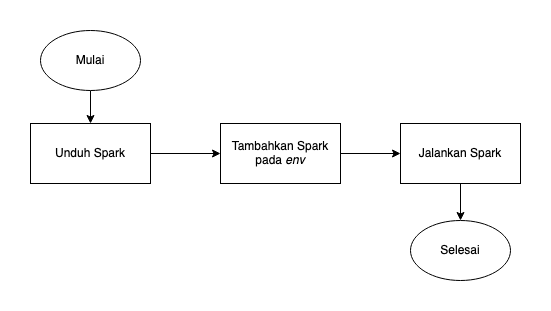
\includegraphics[width=0.7\textwidth]{figures/ch03/spark-flow.png}
    \caption{Alur Instalasi dan Konfigurasi Spark}
    \label{fig:spark-flow}
\end{figure}

\subsection{Instalasi dan Konfigurasi HiBench}
Sebelum melakukan eksperimen, diperlukan suatu perangkat lunak pengukuran kinerja sistem \textit{Big Data}, yaitu HiBench. HiBench tidak dapat digunakan secara langsung ketika sudah berhasil diunduh, melainkan harus dilakukan pembangunan beberapa modul yang dibutuhkan dengan Maven dan konfigurasi beberapa parameter. 

\begin{figure}[h]
    \centering
    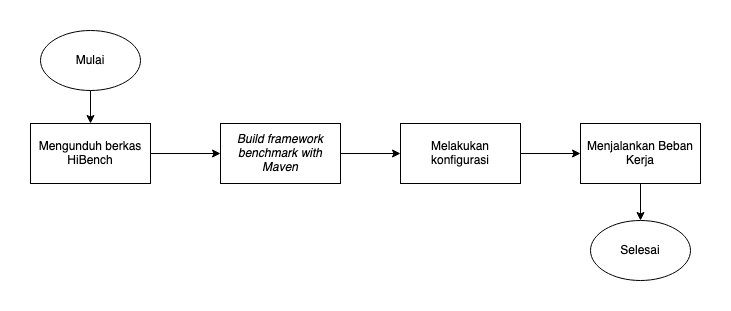
\includegraphics[width=0.9\textwidth]{figures/ch03/hibench-flow.png}
    \caption{Alur Instalasi dan Konfigurasi HiBench}
    \label{fig:hibench-flow}
\end{figure}

Secara umum, alur instalasi dan konfigurasi HiBench sesuai dengan Gambar \ref{fig:hibench-flow}. Berkas HiBench diunduh dari repositori, dilanjutkan dengan pembangunan beberapa modul yang nantinya dibutuhkan. Selanjutnya, dilakukan konfigurasi beberapa berkas seperti \textit{hibench.conf}, hadoop.conf, dan spark.conf. Jika telah dilakukan konfigurasi, dapat dilanjutkan dengan menjalankan beban kerja atau eksperimen. Lebih lanjut, pemasangan dan konfigurasi HiBench dijelaskan pada Lampiran \ref{appendix:E}.

%\begin{table}[]
%\caption{Konfigurasi \textit{HiBench}}
%\label{table:conf-hibench}
%\scriptsize
%\centering
%\begin{tabular}{ll}
%\hline
%\multicolumn{1}{c}{Nama Parameter}  & \multicolumn{1}{c}{Nilai} \\ \hline
%hibench.default.map.parallelism     & 8                         \\
%hibench.default.shuffle.parallelism & 8 \\ \hline                        
%\end{tabular}
%\end{table}


\section{Eksperimen}
Setelah instalasi dan konfigurasi perangkat keras dan perangkat lunak berhasil diselesaikan, tahap selanjutnya adalah eksperimen. Tahap ini melibatkan serangkaian pengujian yang terkontrol untuk mengevaluasi kinerja \textit{platform big data} Hadoop dan Spark dalam menjalankan beban kerja tertentu dengan berbagai ukuran data. Tujuan utama eksperimen ini adalah untuk menjawab pertanyaan penelitian yang telah didefinisikan sebelumnya dan memperoleh pemahaman yang komprehensif tentang karakteristik kinerja masing-masing \textit{platform}.

Penelitian ini difokuskan pada pengujian dua beban kerja yang umum dalam pemrosesan big data, yaitu \textit{word count} dan \textit{sort}. Beban kerja ini akan dieksekusi pada dua \textit{platform big data} yang populer, yaitu Hadoop dan Spark. Setiap kombinasi \textit{platform} dan beban kerja akan diuji dengan 12 ukuran data yang berbeda, mulai dari 100 KB hingga 15 GB. Detail ukuran data yang digunakan ditunjukkan pada Tabel \ref{table:variasi-input-data}. Untuk memastikan reliabilitas dan konsistensi hasil, setiap kombinasi \textit{platform}, beban kerja, dan ukuran data akan diulang sebanyak 5 kali. 

Proses eksperimen menghasilkan dua jenis berkas data: 
\begin{enumerate}
	\item \textit{HiBench Report}: Berisi informasi tentang kinerja beban kerja, termasuk waktu eksekusi, dan \textit{throughput}.
	\item \textit{Dool System Monitoring}: Berisi informasi detail tentang aktivitas sistem selama eksekusi beban kerja, seperti penggunaan CPU, memori, I/O \textit{disk}, dan jaringan.
\end{enumerate}

Secara keseluruhan, desain eksperimen ini menghasilkan 240 percobaan individu, seperti yang diilustrasikan pada Gambar \ref{fig:total-percobaan}. Setiap percobaan mewakili kombinasi unik dari:
\begin{enumerate}
	\item \textit{Platform big data} (Hadoop atau Spark)
	\item Beban kerja (\textit{word count} atau \textit{sort})
	\item Ukuran data (12 variasi)
	\item Pengulangan (5 kali)
\end{enumerate}

\begin{figure}[h]
    \centering
    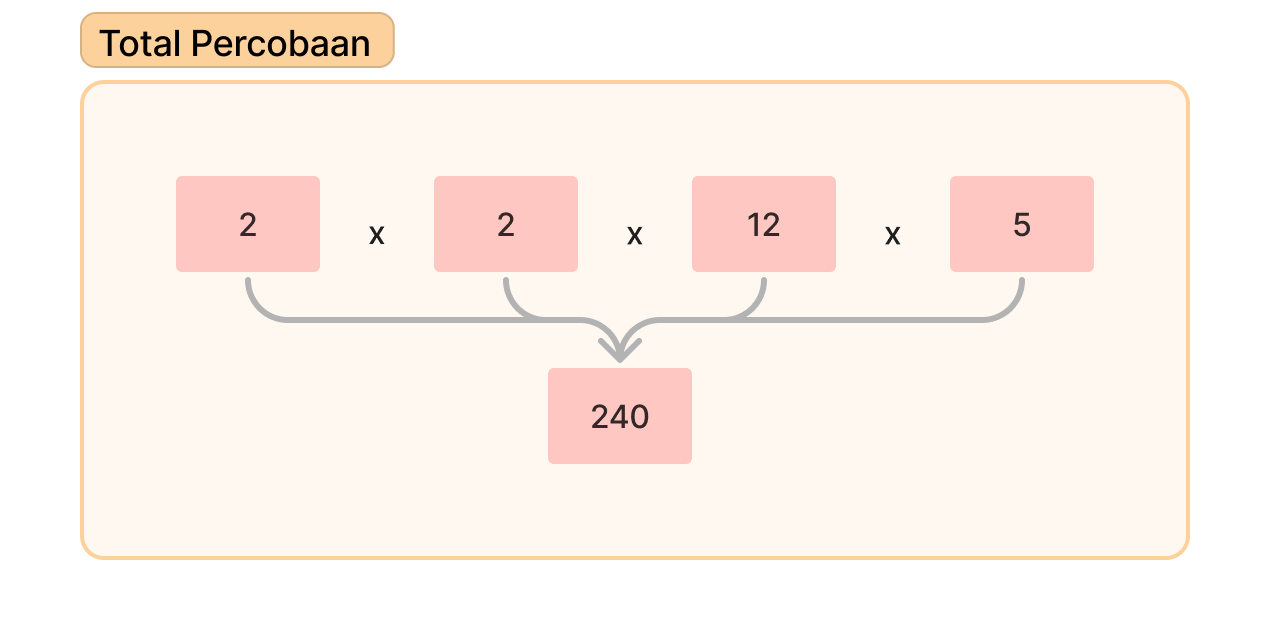
\includegraphics[width=0.7\textwidth]{figures/ch03/total-percobaan.png}
    \caption{Total Percobaan}
    \label{fig:total-percobaan}
\end{figure}

\begin{landscape}
\begin{figure}[h]
    \centering
    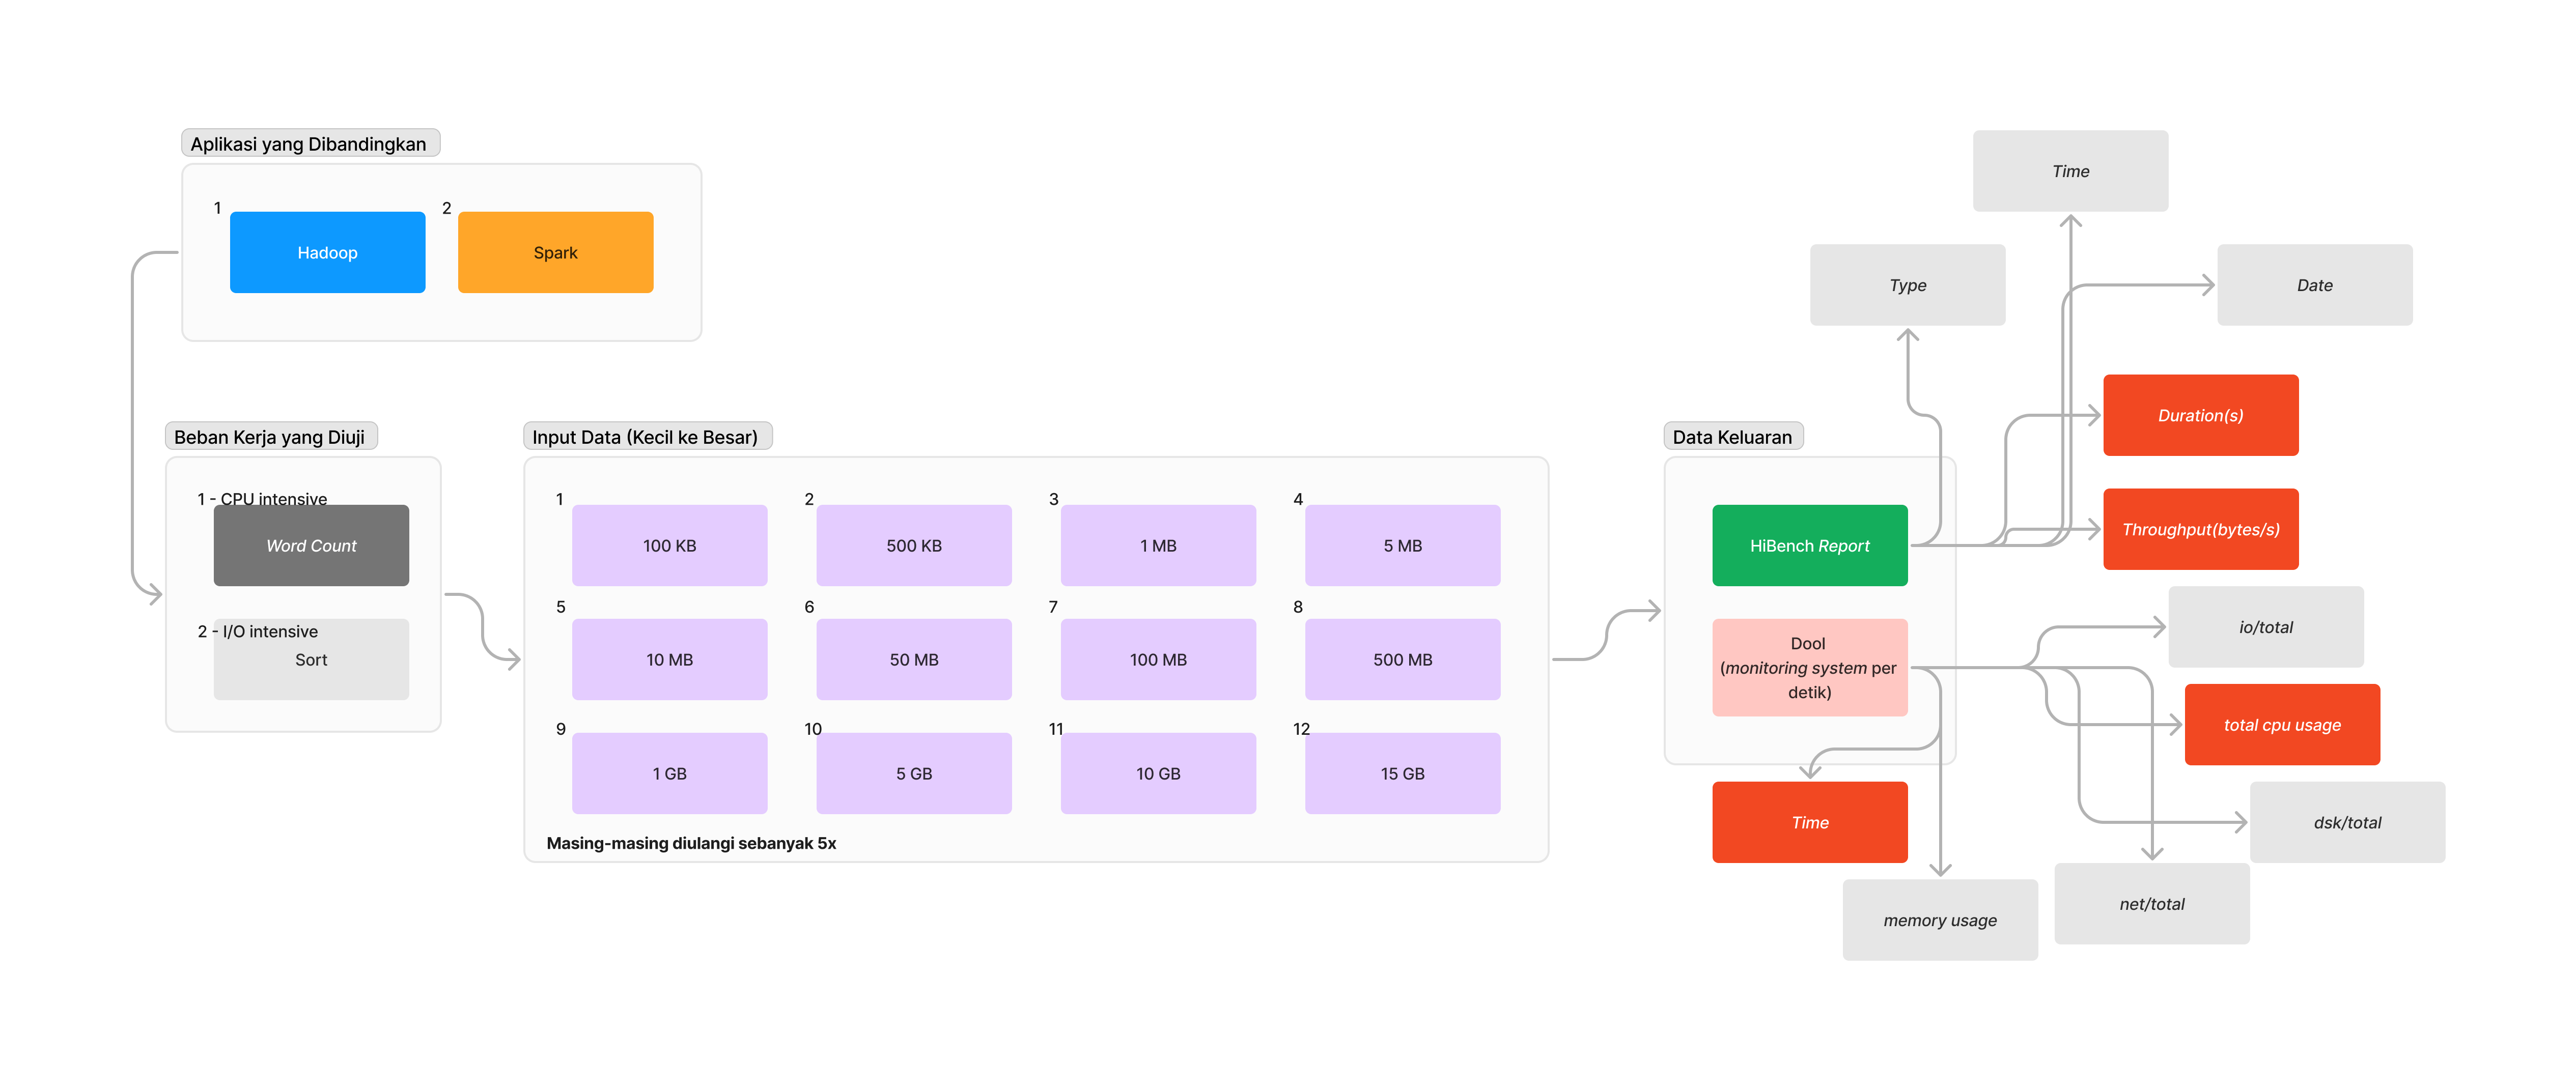
\includegraphics[width=\linewidth, height=0.5\linewidth]{figures/ch03/flow-penelitian-umum.png}
    \caption{\textit{End-to-end} Penelitian}
    \label{fig:flow-penelitian-umum}
\end{figure}
\end{landscape}

Sebagai contoh, untuk \textit{platform} Hadoop dengan beban kerja \textit{word count} dan ukuran data 100 KB, akan menghasilkan lima HiBench \textit{Report} dan lima berkas Dool \textit{System Monitoring}, sesuai dengan jumlah pengulangan.  Ilustrasi ini dapat dilihat pada Gambar \ref{fig:contoh-percobaan}.

\begin{figure}[h]
    \centering
    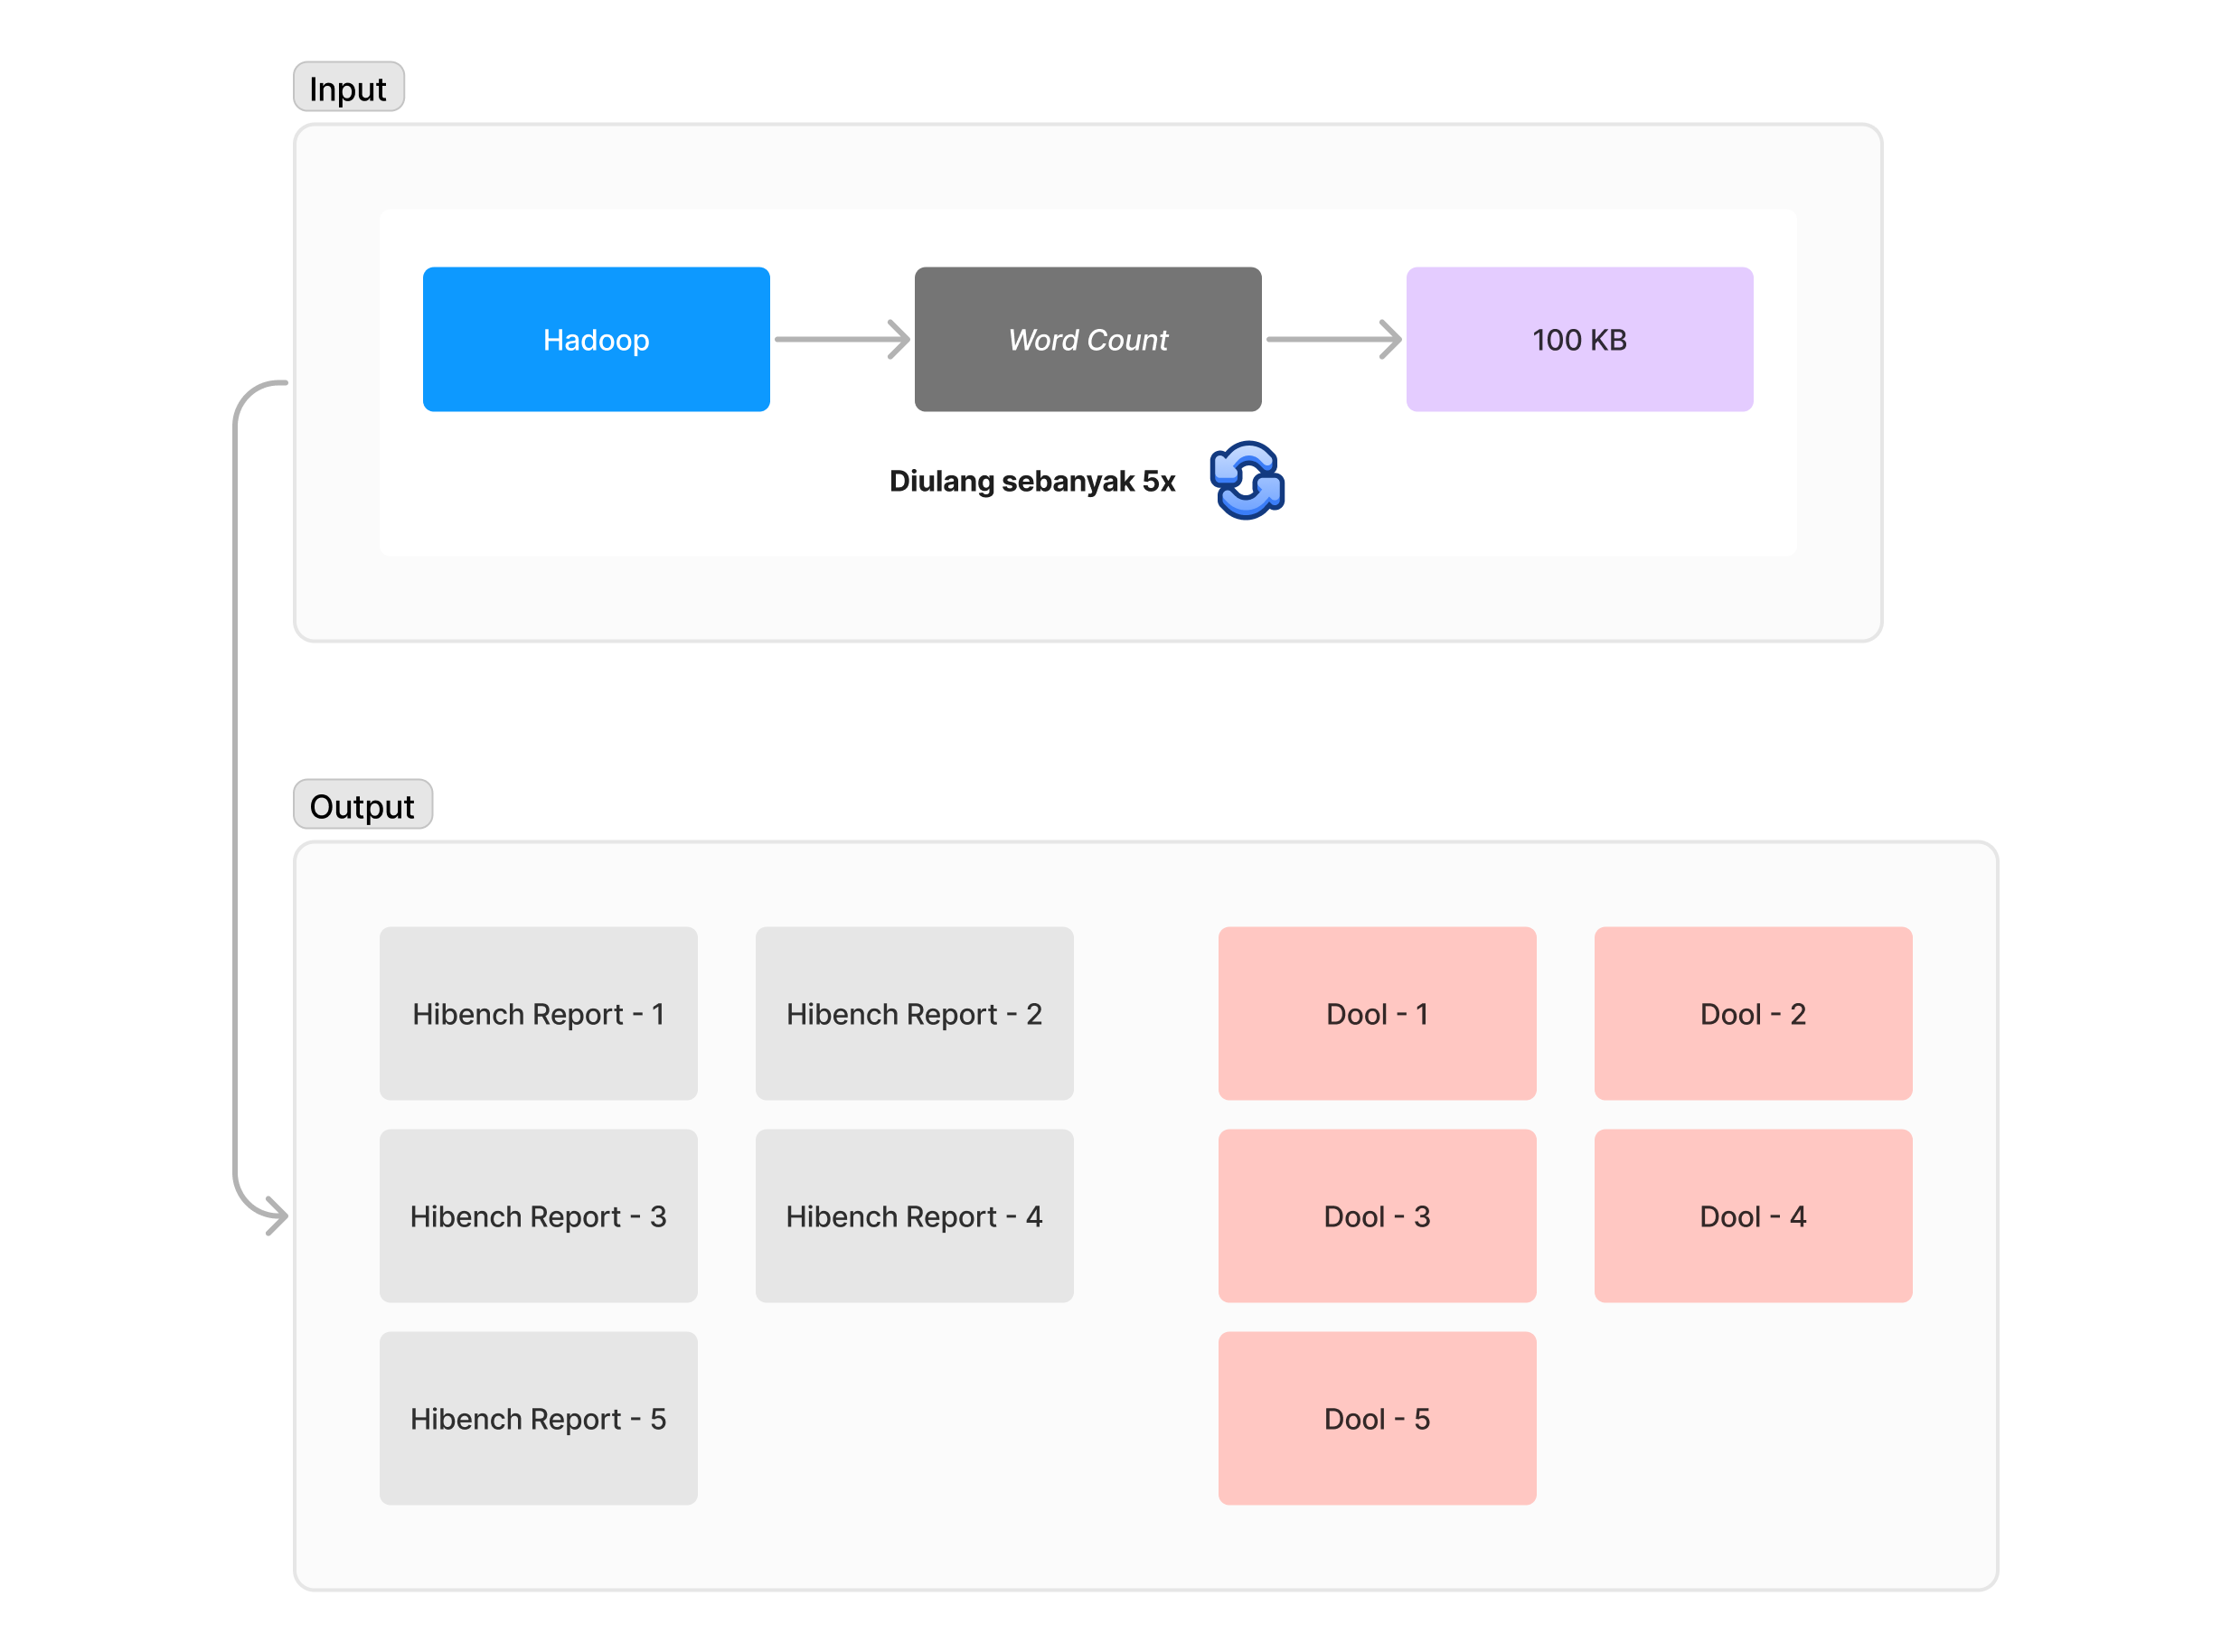
\includegraphics[width=0.9\textwidth]{figures/ch03/contoh-percobaan.png}
    \caption{Contoh Percobaan}
    \label{fig:contoh-percobaan}
\end{figure}

\begin{table}[]
\caption{Variasi Input Data}
\label{table:variasi-input-data}
\centering
\begin{tabular}{lll}
\hline
\multicolumn{1}{c}{\textbf{No}} & \multicolumn{1}{c}{\textbf{Label Input Data}} & \multicolumn{1}{c}{\begin{tabular}[c]{@{}c@{}}\textbf{Ukuran Input Data  (bita)}\end{tabular}} \\ \hline
1  & 100 KB & 100000 ($1 * 10^5$) \\
2  & 500 KB & 500000 ($5 * 10^5$) \\
3  & 1 MB   & $1 * 10^6$          \\
4  & 5 MB   & $5 * 10^6$          \\
5  & 10 MB  & $1 * 10^7$          \\
6  & 50 MB  & $5 * 10^7$          \\
7  & 100 MB & $1 * 10^8$          \\
8  & 500 MB & $5 * 10^8$          \\
9  & 1 GB   & $1 * 10^9$          \\
10 & 5 GB   & $5 * 10^9$          \\
11 & 10 GB  & $1 * 10^{10}$         \\ 
12 & 15 GB  & $1.5 * 10^{10}$       \\ \hline
\end{tabular}
\end{table}


Karena jumlah percobaan yang banyak, otomatisasi menjadi penting untuk memastikan efisiensi dan akurasi.  Skrip khusus dikembangkan untuk mengotomatiskan seluruh proses eksperimen, termasuk konfigurasi HiBench, persiapan data, eksekusi beban kerja, dan pengumpulan data. Detail skrip otomatisasi dapat ditemukan pada Lampiran \ref{appendix:F}.

Algoritma otomatisasi eksperimen dimulai dengan mengubah direktori kerja ke direktori HiBench.  Selanjutnya, algoritma melakukan iterasi untuk setiap beban kerja yang ditentukan.  Di dalam setiap iterasi beban kerja, dilakukan iterasi lagi untuk setiap ukuran data.  Pada setiap kombinasi beban kerja dan ukuran data, konfigurasi HiBench diubah sesuai dengan ukuran data yang dipilih.

Skrip persiapan data Hadoop dan Spark dijalankan berulang kali hingga proses persiapan berhasil.  Setelah data siap, perulangan dilakukan sebanyak jumlah pengulangan yang ditentukan.  Dalam setiap perulangan, perangkat lunak "dool" diaktifkan untuk memonitor aktivitas sistem, \textit{benchmark} Hadoop atau Spark dijalankan, dan monitoring sistem dihentikan.

Setelah semua perulangan selesai, algoritma menunggu selama 15 detik sebelum melanjutkan ke ukuran data berikutnya. Proses ini berlanjut hingga semua kombinasi beban kerja dan ukuran data selesai diproses.

\section{Analisis dan Evaluasi Hasil Eksperimen}

Setelah menyelesaikan 240 percobaan yang dijelaskan di bagian eksperimen, langkah selanjutnya adalah menganalisis dan mengevaluasi hasil yang diperoleh. Analisis ini bertujuan untuk menjawab pertanyaan penelitian dan memahami bagaimana kinerja Hadoop dan Spark dalam menjalankan beban kerja \textit{word count} dan \textit{sort} dengan berbagai ukuran data. Berikut adalah beberapa aspek yang akan dikaji:

\begin{enumerate}	
	\item \textbf{Kinerja}
	\begin{enumerate}
		\item \textbf{Persebaran Waktu Eksekusi pada Hadoop dan Spark}. Bagian ini akan menganalisis sebaran waktu eksekusi untuk setiap beban kerja (\textit{word count} dan \textit{sort}) pada kedua aplikasi (Hadoop dan Spark) dengan berbagai ukuran data. Analisis ini akan membantu memahami variabilitas kinerja dan konsistensi hasil pada setiap kombinasi aplikasi, beban kerja, dan ukuran data.
		\item \textbf{Persebaran \textit{Throughput} pada Hadoop dan Spark}. Mirip dengan analisis waktu eksekusi, persebaran \textit{throughput} juga akan dianalisis untuk setiap kombinasi aplikasi, beban kerja, dan ukuran data. Throughput, yang menunjukkan jumlah data yang diproses per satuan waktu,  merupakan metrik penting dalam evaluasi kinerja sistem big data.  Visualisasi distribusi throughput akan membantu dalam memahami efisiensi pemrosesan data oleh Hadoop dan Spark.
		\item \textbf{Rata-rata Waktu Eksekusi pada Hadoop dan Spark}. Selain persebaran, rata-rata waktu eksekusi untuk setiap kombinasi akan dihitung dan dibandingkan.  Ini memberikan gambaran umum tentang kinerja relatif setiap aplikasi dalam menyelesaikan beban kerja tertentu dengan ukuran data tertentu. Perbedaan rata-rata waktu eksekusi antara Hadoop dan Spark, serta tren perubahannya seiring dengan peningkatan ukuran data, akan diidentifikasi dan dibahas.
		\item \textbf{Rata-rata \textit{Throughput} pada Hadoop dan Spark}. Serupa dengan rata-rata waktu eksekusi, rata-rata \textit{throughput} juga akan dihitung dan dibandingkan untuk setiap kombinasi. Analisis ini membantu memahami bagaimana efisiensi pemrosesan data berubah dengan berbagai beban kerja dan ukuran data, serta memberikan wawasan tentang skalabilitas setiap platform.
		\item \textbf{\textit{Rate of Change}}. \textit{Rate of Change} akan dihitung untuk metrik-metrik kinerja seperti waktu eksekusi dan \textit{throughput}. Analisis ini akan menunjukkan seberapa besar perubahan kinerja seiring dengan peningkatan ukuran data.  
	\end{enumerate}
	\item \textbf{Penggunaan Sumber Daya}
	\begin{enumerate}
	\item \textbf{Penggunaan CPU}. Bagian ini akan menganalisis penggunaan CPU oleh Hadoop dan Spark selama menjalankan berbagai beban kerja.  Informasi ini dapat diperoleh dari berkas monitoring sistem yang dihasilkan oleh Dool.  Analisis penggunaan CPU membantu memahami bagaimana setiap platform memanfaatkan sumber daya komputasi dan mengidentifikasi potensi optimasi.
	\item \textbf{Utilisasi Sistem}. Selain penggunaan CPU, metrik-metrik lain seperti penggunaan memori, dan I/O penyimpanan. Hal ini memberikan gambaran yang lebih komprehensif tentang bagaimana setiap \textit{platform} memanfaatkan sumber daya sistem dan potensi \textit{bottleneck} yang mungkin terjadi selama pemrosesan data besar.
	\end{enumerate}
\end{enumerate}











